\documentclass[12pt]{article}
\usepackage[utf8]{inputenc}   % UTF-8 encoding
\usepackage{amsmath}          % For advanced math
\usepackage{amssymb}          % For symbols
\usepackage{geometry}         % To adjust margins
\usepackage{graphicx}         % For including images
\usepackage{hyperref}         % For clickable links
\usepackage{physics}          % Optional: easy physics notation
\usepackage{caption}          % Better captions
\usepackage{subcaption}
\usepackage{enumitem}         % Custom lists
\usepackage{titlesec}         % Customize section titles
\usepackage{float}

% Table
\usepackage[table]{xcolor}
\usepackage{colortbl}
\usepackage{array}
\usepackage{makecell}

% Codeblocks
\usepackage{listings}

\lstset{
	numbers=left,
	tabsize=1,
	tab=1,
	xleftmargin=1pt,
	basicstyle=\ttfamily,
	breaklines=true,
	frame=single,
}

% ---------- Page Setup ----------
\geometry{
	a4paper,
	left=25mm,
	right=25mm,
	top=25mm,
	bottom=25mm
}

% ---------- Title Info ----------
\title{
	\textbf{Principles of Data Communications and Networks Modeling (CS4865/6865)} \\[2mm]
	\textbf{}
	\text{Lab Report \#1: Introduction to network simulation I}
}
\author{Abid Hasan Muin (3804634)}
\date{Due date: September 29, 2025}

% ---------- Section formatting ----------
\titleformat{\section}{\large\bfseries}{Exercise \thesection:}{1em}{}
\setcounter{section}{0}  % Start numbering from 1

\begin{document}
	
	\maketitle
	
	% Exercise 2
	
	\setcounter{section}{1}
	\section{}	
	
	\subsection{Code}
	\begin{lstlisting}[language=Tcl]
		set ns [new Simulator]
		
		set nf [open exer_2.nam w]
		$ns namtrace-all $nf
		
		proc finish {} {
			global ns nf
			$ns flush-trace
			close $nf
			exec nam exer_2.nam &
			exit 0
		}
		
		set n0 [$ns node]
		set n1 [$ns node]
		
		$ns duplex-link $n0 $n1 1Mb 10ms DropTail
		
		set udp0 [new Agent/UDP]
		$ns attach-agent $n0 $udp0
		
		set cbr0 [new Application/Traffic/CBR]
		$cbr0 set packetSize_ 500
		$cbr0 set interval_ 0.005
		$cbr0 attach-agent $udp0		
		
		set null0 [new Agent/Null] 
		$ns attach-agent $n1 $null0
		
		$ns connect $udp0 $null0
		
		$ns at 0.5 "$cbr0 start"
		$ns at 4.5 "$cbr0 stop"
		
		$ns at 5.0 "finish"
		
		$ns run
	\end{lstlisting}
	
	\subsection{NAM Screenshot}
	
	\begin{figure}[htbp]
		\centering
		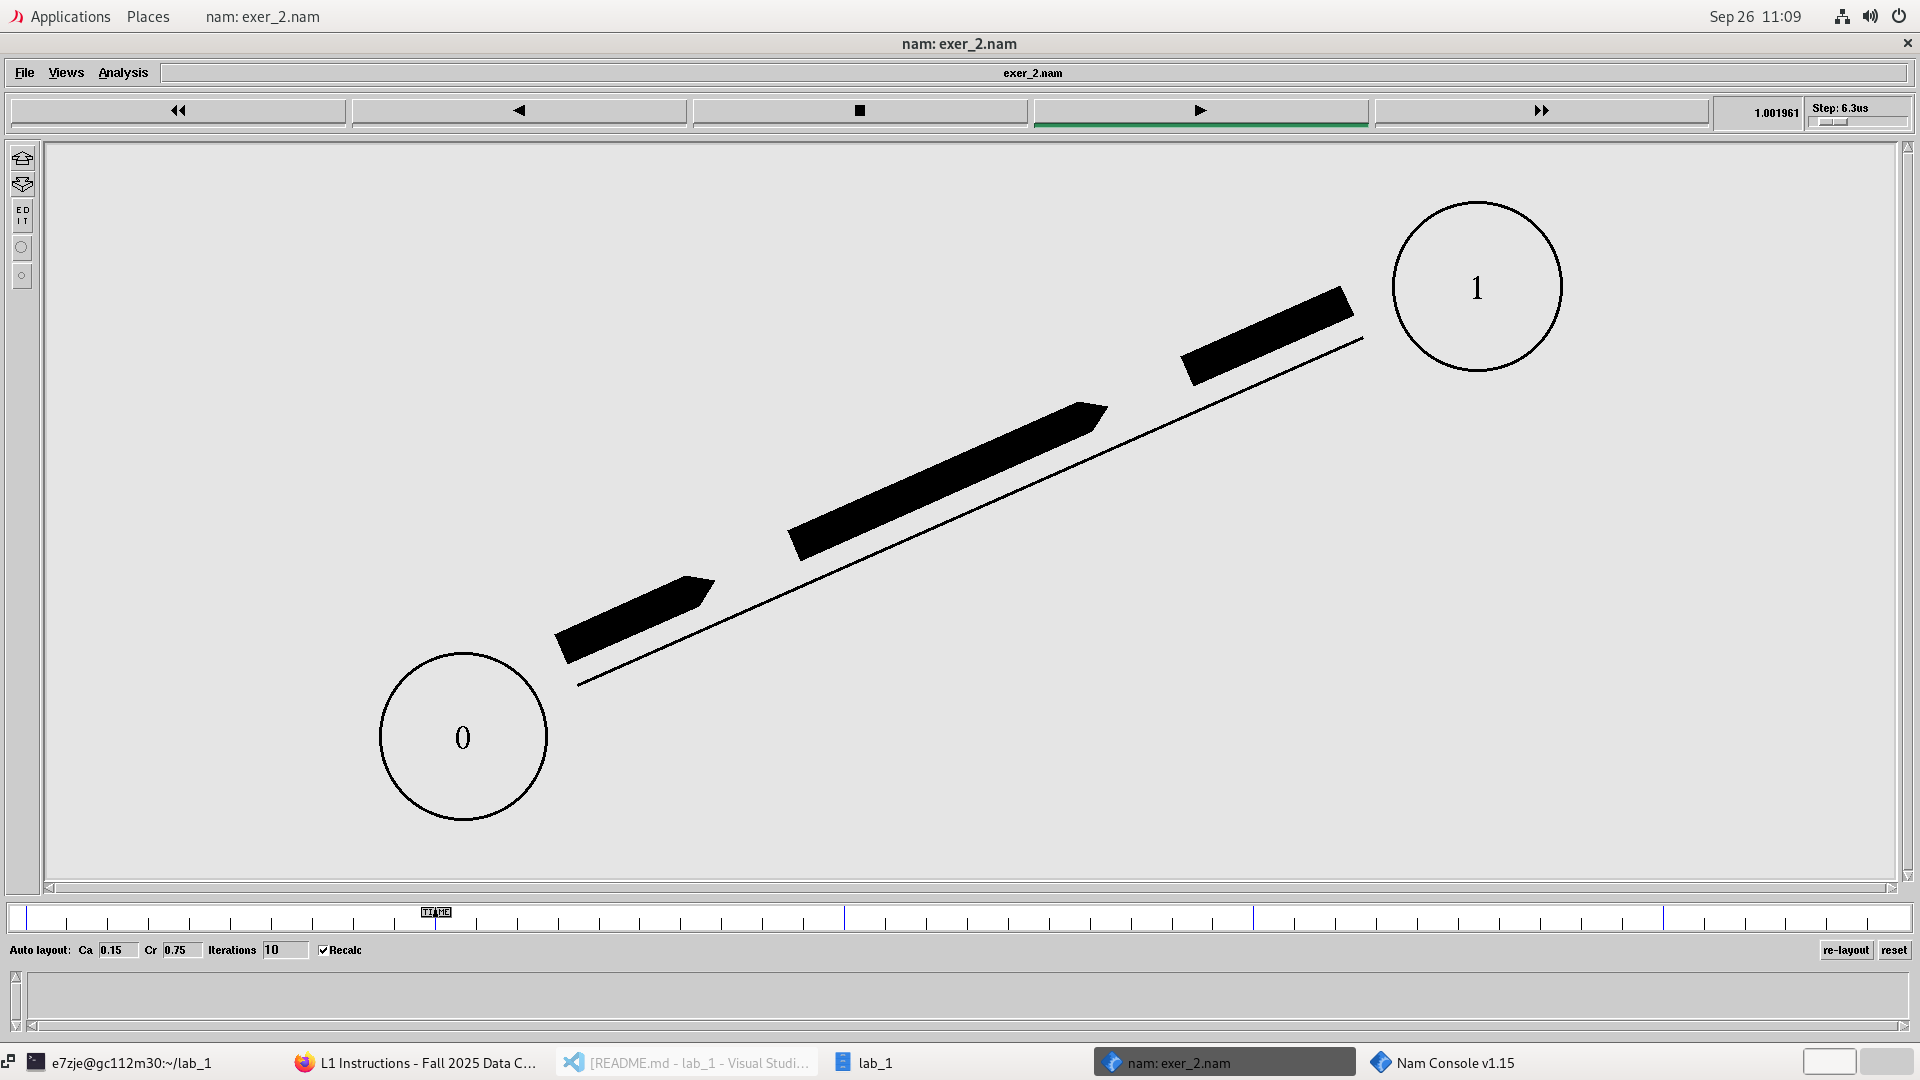
\includegraphics[width=\textwidth]{lab_1/exer_2.png}
		\caption{NAM Screenshot of Exercise 2}
		\label{fig:graph}
	\end{figure}
	
	% Exercise 3
	\section{}
	\subsection{Trace file}
	
	\begin{lstlisting}[]
		V -t * -v 1.0a5 -a 0
		A -t * -n 1 -p 0 -o 0x7fffffff -c 30 -a 1
		A -t * -h 1 -m 1073741823 -s 0
		n -t * -a 0 -s 0 -S UP -v circle -c black -i black
		n -t * -a 1 -s 1 -S UP -v circle -c black -i black
		l -t * -s 0 -d 1 -S UP -r 1000000 -D 0.01 -c black
		+ -t 0.5 -s 0 -d 1 -p cbr -e 500 -c 0 -i 0 -a 0 -x {0.0 1.0 0 ------- null}
		- -t 0.5 -s 0 -d 1 -p cbr -e 500 -c 0 -i 0 -a 0 -x {0.0 1.0 0 ------- null}
		h -t 0.5 -s 0 -d 1 -p cbr -e 500 -c 0 -i 0 -a 0 -x {0.0 1.0 -1 ------- null}
		+ -t 0.505 -s 0 -d 1 -p cbr -e 500 -c 0 -i 1 -a 0 -x {0.0 1.0 1 ------- null}
		- -t 0.505 -s 0 -d 1 -p cbr -e 500 -c 0 -i 1 -a 0 -x {0.0 1.0 1 ------- null}
		h -t 0.505 -s 0 -d 1 -p cbr -e 500 -c 0 -i 1 -a 0 -x {0.0 1.0 -1 ------- null}
		+ -t 0.51 -s 0 -d 1 -p cbr -e 500 -c 0 -i 2 -a 0 -x {0.0 1.0 2 ------- null}
		- -t 0.51 -s 0 -d 1 -p cbr -e 500 -c 0 -i 2 -a 0 -x {0.0 1.0 2 ------- null}
		h -t 0.51 -s 0 -d 1 -p cbr -e 500 -c 0 -i 2 -a 0 -x {0.0 1.0 -1 ------- null}
		r -t 0.514 -s 0 -d 1 -p cbr -e 500 -c 0 -i 0 -a 0 -x {0.0 1.0 0 ------- null}
		+ -t 0.515 -s 0 -d 1 -p cbr -e 500 -c 0 -i 3 -a 0 -x {0.0 1.0 3 ------- null}
		- -t 0.515 -s 0 -d 1 -p cbr -e 500 -c 0 -i 3 -a 0 -x {0.0 1.0 3 ------- null}
		h -t 0.515 -s 0 -d 1 -p cbr -e 500 -c 0 -i 3 -a 0 -x {0.0 1.0 -1 ------- null}
		r -t 0.519 -s 0 -d 1 -p cbr -e 500 -c 0 -i 1 -a 0 -x {0.0 1.0 1 ------- null}
		+ -t 0.52 -s 0 -d 1 -p cbr -e 500 -c 0 -i 4 -a 0 -x {0.0 1.0 4 ------- null}
		- -t 0.52 -s 0 -d 1 -p cbr -e 500 -c 0 -i 4 -a 0 -x {0.0 1.0 4 ------- null}
		h -t 0.52 -s 0 -d 1 -p cbr -e 500 -c 0 -i 4 -a 0 -x {0.0 1.0 -1 ------- null}
		r -t 0.524 -s 0 -d 1 -p cbr -e 500 -c 0 -i 2 -a 0 -x {0.0 1.0 2 ------- null}
		+ -t 0.525 -s 0 -d 1 -p cbr -e 500 -c 0 -i 5 -a 0 -x {0.0 1.0 5 ------- null}
		- -t 0.525 -s 0 -d 1 -p cbr -e 500 -c 0 -i 5 -a 0 -x {0.0 1.0 5 ------- null}
		h -t 0.525 -s 0 -d 1 -p cbr -e 500 -c 0 -i 5 -a 0 -x {0.0 1.0 -1 ------- null}
		r -t 0.529 -s 0 -d 1 -p cbr -e 500 -c 0 -i 3 -a 0 -x {0.0 1.0 3 ------- null}
		+ -t 0.53 -s 0 -d 1 -p cbr -e 500 -c 0 -i 6 -a 0 -x {0.0 1.0 6 ------- null}
		- -t 0.53 -s 0 -d 1 -p cbr -e 500 -c 0 -i 6 -a 0 -x {0.0 1.0 6 ------- null}
	\end{lstlisting}

	\subsection{First Packet Transmitted}
	The first packet being transmitted can be seen in line number 7.
	\newline
	\texttt{+ -t 0.5 -s 0 -d 1 -p cbr -e 500 -c 0 -i 0 -a 0 -x \{0.0 1.0 0 ------- null\}}
	
	\subsection{First Packet Received}
	The first packet being transmitted can be seen in line number 16.
	\newline
	\texttt{r -t 0.514 -s 0 -d 1 -p cbr -e 500 -c 0 -i 0 -a 0 -x \{0.0 1.0 0 ------- null\}}
	
	% Exercise 4
	\section{}	
	
	\subsection{Code}
	\begin{lstlisting}[language=Tcl]
		set ns [new Simulator]
		
		set nf [open exer_4.nam w]
		$ns namtrace-all $nf
		
		set n0 [$ns node]
		set n1 [$ns node]
		set n2 [$ns node]
		
		$ns duplex-link $n0 $n1 1Mb 10ms DropTail
		$ns duplex-link $n1 $n2 1Mb 10ms DropTail
		
		set udp0 [new Agent/UDP]
		$ns attach-agent $n0 $udp0
		
		set cbr0 [new Application/Traffic/CBR]
		$cbr0 set packetSize_ 500
		$cbr0 set interval_ 0.005
		$cbr0 attach-agent $udp0
		
		
		set null0 [new Agent/Null] 
		$ns attach-agent $n2 $null0
		
		$ns connect $udp0 $null0
		
		$ns at 0.5 "$cbr0 start"
		$ns at 4.5 "$cbr0 stop"
		
		proc finish {} {
			global ns nf
			$ns flush-trace
			close $nf
			exec nam exer_4.nam &
			exit 0
		}
		
		$ns at 5.0 "finish"
		
		$ns run
	\end{lstlisting}
	
	\subsection{NAM Screenshot}
	
	\begin{figure}[htbp]
		\centering
		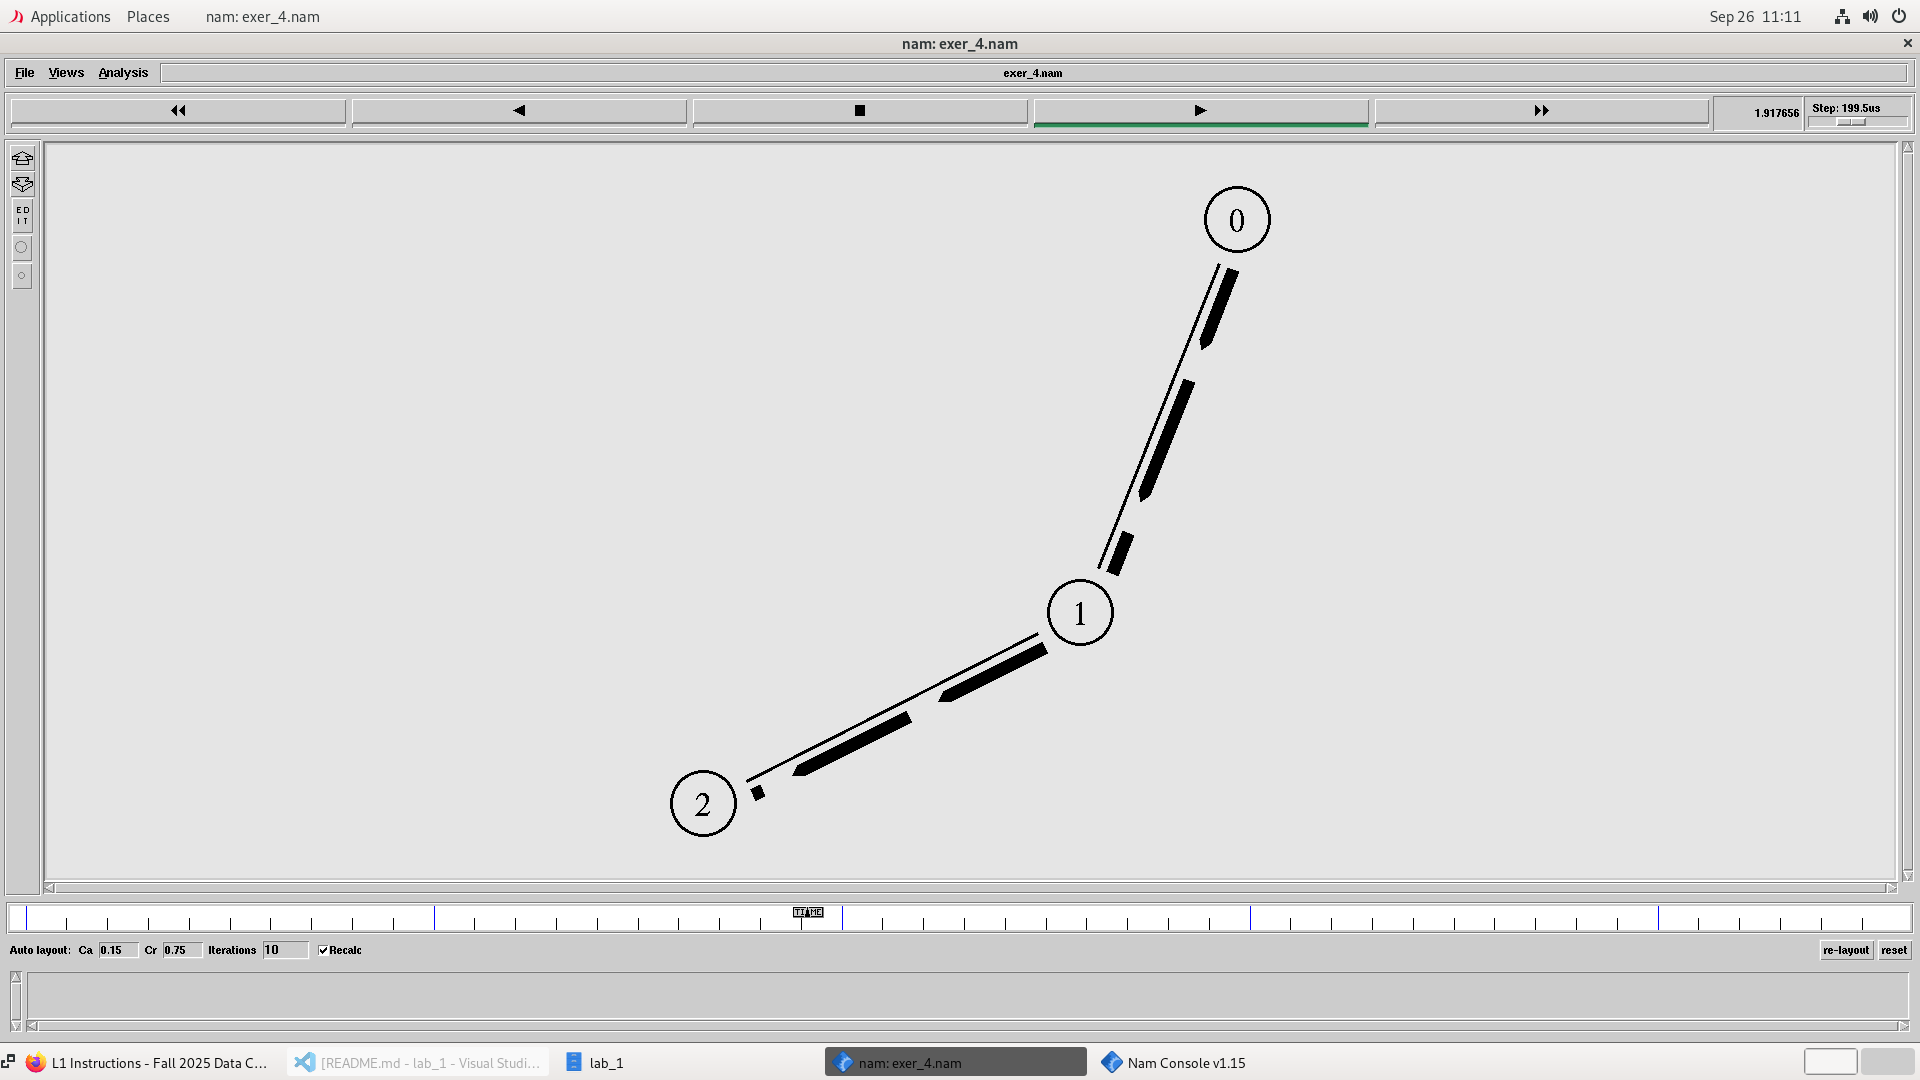
\includegraphics[width=\textwidth]{lab_1/exer_4.png}
		\caption{NAM Screenshot of Exercise 4}
		\label{fig:graph1}
	\end{figure}
	
	% Exercise 5
	\section{}
	\subsection{Trace file}
	
	\begin{lstlisting}[]
		V -t * -v 1.0a5 -a 0
		A -t * -n 1 -p 0 -o 0x7fffffff -c 30 -a 1
		A -t * -h 1 -m 1073741823 -s 0
		n -t * -a 0 -s 0 -S UP -v circle -c black -i black
		n -t * -a 1 -s 1 -S UP -v circle -c black -i black
		n -t * -a 2 -s 2 -S UP -v circle -c black -i black
		l -t * -s 0 -d 1 -S UP -r 1000000 -D 0.01 -c black
		l -t * -s 1 -d 2 -S UP -r 1000000 -D 0.01 -c black
		+ -t 0.5 -s 0 -d 1 -p cbr -e 500 -c 0 -i 0 -a 0 -x {0.0 2.0 0 ------- null}
		- -t 0.5 -s 0 -d 1 -p cbr -e 500 -c 0 -i 0 -a 0 -x {0.0 2.0 0 ------- null}
		h -t 0.5 -s 0 -d 1 -p cbr -e 500 -c 0 -i 0 -a 0 -x {0.0 2.0 -1 ------- null}
		+ -t 0.505 -s 0 -d 1 -p cbr -e 500 -c 0 -i 1 -a 0 -x {0.0 2.0 1 ------- null}
		- -t 0.505 -s 0 -d 1 -p cbr -e 500 -c 0 -i 1 -a 0 -x {0.0 2.0 1 ------- null}
		h -t 0.505 -s 0 -d 1 -p cbr -e 500 -c 0 -i 1 -a 0 -x {0.0 2.0 -1 ------- null}
		+ -t 0.51 -s 0 -d 1 -p cbr -e 500 -c 0 -i 2 -a 0 -x {0.0 2.0 2 ------- null}
		- -t 0.51 -s 0 -d 1 -p cbr -e 500 -c 0 -i 2 -a 0 -x {0.0 2.0 2 ------- null}
		h -t 0.51 -s 0 -d 1 -p cbr -e 500 -c 0 -i 2 -a 0 -x {0.0 2.0 -1 ------- null}
		r -t 0.514 -s 0 -d 1 -p cbr -e 500 -c 0 -i 0 -a 0 -x {0.0 2.0 0 ------- null}
		+ -t 0.514 -s 1 -d 2 -p cbr -e 500 -c 0 -i 0 -a 0 -x {0.0 2.0 0 ------- null}
		- -t 0.514 -s 1 -d 2 -p cbr -e 500 -c 0 -i 0 -a 0 -x {0.0 2.0 0 ------- null}
		h -t 0.514 -s 1 -d 2 -p cbr -e 500 -c 0 -i 0 -a 0 -x {0.0 2.0 -1 ------- null}
		+ -t 0.515 -s 0 -d 1 -p cbr -e 500 -c 0 -i 3 -a 0 -x {0.0 2.0 3 ------- null}
		- -t 0.515 -s 0 -d 1 -p cbr -e 500 -c 0 -i 3 -a 0 -x {0.0 2.0 3 ------- null}
		h -t 0.515 -s 0 -d 1 -p cbr -e 500 -c 0 -i 3 -a 0 -x {0.0 2.0 -1 ------- null}
		r -t 0.519 -s 0 -d 1 -p cbr -e 500 -c 0 -i 1 -a 0 -x {0.0 2.0 1 ------- null}
		+ -t 0.519 -s 1 -d 2 -p cbr -e 500 -c 0 -i 1 -a 0 -x {0.0 2.0 1 ------- null}
		- -t 0.519 -s 1 -d 2 -p cbr -e 500 -c 0 -i 1 -a 0 -x {0.0 2.0 1 ------- null}
		h -t 0.519 -s 1 -d 2 -p cbr -e 500 -c 0 -i 1 -a 0 -x {0.0 2.0 -1 ------- null}
		+ -t 0.52 -s 0 -d 1 -p cbr -e 500 -c 0 -i 4 -a 0 -x {0.0 2.0 4 ------- null}
		- -t 0.52 -s 0 -d 1 -p cbr -e 500 -c 0 -i 4 -a 0 -x {0.0 2.0 4 ------- null}
	\end{lstlisting}
	
	\subsection{First Packet Transmitted}
	The first packet being transmitted can be seen in line number 9 and the time stamp is 0.5
	\newline
	\texttt{+ -t 0.5 -s 0 -d 1 -p cbr -e 500 -c 0 -i 0 -a 0 -x \{0.0 2.0 0 ------- null\}}
	
	\subsection{First Packet Received at Forwarding Node}
	The first packet being received at forwarding node can be seen in line number 18 and the time stamp is 0.514
	\newline
	\texttt{r -t 0.514 -s 0 -d 1 -p cbr -e 500 -c 0 -i 0 -a 0 -x \{0.0 2.0 0 ------- null\}}
	
	\subsection{First Packet Received at Destination Node}
	The first packet being received at destination node can be seen in line number 39 and the time stamp is 0.528
	\newline
	\texttt{r -t 0.528 -s 1 -d 2 -p cbr -e 500 -c 0 -i 0 -a 0 -x \{0.0 2.0 0 ------- null\}}
	
	
	\subsection{Delivery Time Calculation}
		\textbf{From trace data:}
		\begin{itemize}
			\item {Destination receive time =} 0.528 seconds
			\item {Source transmission time =} 0.5 seconds (enqueue time represents when transmission begins)
		\end{itemize}
		
		\noindent
		The total delivery time of a packet from the source node to the destination node can be calculated using the following formula:
		
		\begin{align*}
			\text{Delivery Time} &= \text{Destination Receive Time} - \text{Source Transmission Time} \\
			&= 0.528 - 0.5 \\
			&= 0.028 \text{ seconds}
		\end{align*}

		\noindent		
		This delivery time is derived from the timestamps in the trace file, which show the complete path of the packet:
		
		\begin{enumerate}
			\item Packet 0 is enqueued at node 0 at 0.5 seconds.
			\item Packet 0 is received at node 1 (the forwarding node) at 0.514 seconds.
			\item Packet 0 is received at node 2 (the destination node) at 0.528 seconds.
		\end{enumerate}
		
		\noindent
		The total time includes the transmission delays from node 0 to node 1 and from node 1 to node 2, along with any processing delays at the intermediate node.
		
		\noindent
		\newline
		This analysis represents a simple three-node topology, where node 0 is the source, node 1 is the intermediate forwarding node, and node 2 is the destination. The traffic is CBR (Constant Bit Rate), and the packet flows from node 0 to node 2 via node 1.
	
	% Exercise 6
	\section{Theoretical Delay Calculation}
	\subsection{Network Parameters from the Trace File}
	
	From the trace, we can extract:
	\begin{verbatim}
	Link 0 -> 1: l -t * -s 0 -d 1 -S UP -r 1000000 -D 0.01 -c black
	Link 1 -> 2: l -t * -s 1 -d 2 -S UP -r 1000000 -D 0.01 -c black
	Packet size: 500 bytes (from -e 500 in packet events)
	\end{verbatim}
	Key parameters:
	\begin{verbatim}
	Link bandwidth (rate): 1,000,000 bps (1 Mbps)
	Link propagation delay: 0.01 seconds
	Packet size: 500 bytes = 4,000 bits
	\end{verbatim}
	
	
	\subsection{Delay Components Formula}
	Total delay = Transmission delay + Propagation delay + Processing delay + Queuing delay
	
	\noindent
	For our case:
	\begin{itemize}
		\item Processing delay is typically negligible in NS-2 unless specified.
		\item Queuing delay should be zero for the first packet (no packets ahead in queue)
	\end{itemize}
	
	\begin{equation*}
		\text{Transmission delay} = \frac{\text{Packet size}}{\text{Bandwidth}}
	\end{equation*}

	\begin{equation*}
		\text{Propagation delay} = \frac{\text{Distance}}{\text{Propagation speed}}
	\end{equation*}
	
	
	\subsection{Theoretical Calculation}
	For one hop (node 0 $\rightarrow$ node 1):
	
	\begin{align*}
		\text{Transmission delay} &= \frac{4000~\mathrm{bits}}{1,000,000~\mathrm{bps}} \\
		&= 0.004 \text{ seconds}
	\end{align*}
	
	\noindent
	Propagation delay = 0.01 seconds \\
	Total per hop delay = 0.004 + 0.01 = 0.014 seconds
	
	\noindent
	\newline
	For two hops (node 0 $\rightarrow$ node 1 $\rightarrow$ node 2):
	
	\begin{verbatim}
		Hop 1 (0 -> 1): 0.014 seconds
		Hop 2 (1 -> 2): 0.014 seconds
	\end{verbatim}
	
	\noindent
	Total theoretical delay = 0.014 + 0.014 = 0.028 seconds
	
	\subsection{Comparison with Empirical Measurement}
	Empirical delay measured = 0.528s - 0.5s = 0.028 seconds \\
	Theoretical delay (0.028s) = Empirical delay (0.028s) \\
	Yes, this calculated delay is same as the delay value which was calculated in Exercise 5.2

	\begin{thebibliography}{9}
		\bibitem{mark} Mark Greis, Tutorial for the Network Simulator "ns": \url{http://www.isi.edu/nsnam/ns/tutorial/index.html}
		\bibitem{tcl} TCL description: \url{http://en.wikipedia.org/wiki/Tcl}
		\bibitem{ns} ns manual: \url{https://www.isi.edu/nsnam/ns/ns-documentation.html}
		\bibitem{trace} Trace file format: \url{https://www.isi.edu/websites/nsnam/ns/doc/node289.html}
		\bibitem{nam} nam trace file format: \url{https://www.isi.edu/websites/nsnam/ns/doc/node616.html}
	\end{thebibliography}
\end{document}